% Supplementary Information of the HPO paper
% September 2016

\documentclass{bioinfo}
\copyrightyear{2015} \pubyear{2015}

\access{Advance Access Publication Date: Day Month Year}
\appnotes{Manuscript Category}

\usepackage{fancybox}
%\usepackage{enumitem}

%% diagonal line in a cell table
%\usepackage{slashbox}

%\setcounter{secnumdepth}{6}

\usepackage{multirow} 
\usepackage[table]{xcolor}
\definecolor{lightgray}{gray}{0.9}

%% cross referencing with Main Paper (HPOmain.tex)
\usepackage{hyperref}
\usepackage{xr}
\externaldocument{HPOMain}

\newcommand{\inda}{\phantom{1}\hspace{3mm}}
\newcommand{\indb}{\phantom{1}\hspace{8.5mm}}
\newcommand{\indc}{\phantom{1}\hspace{12mm}}
\newcommand{\indd}{\phantom{1}\hspace{16mm}}
\newcommand{\inde}{\phantom{1}\hspace{20mm}}
\newcommand{\indf}{\phantom{1}\hspace{24mm}}
\newcommand{\indg}{\phantom{1}\hspace{28mm}}
\newcommand{\indh}{\phantom{1}\hspace{32mm}}
\newcommand{\bs}{\boldsymbol{s}}

\newcommand{\by}{\boldsymbol{y}}
\newcommand{\bt}{\boldsymbol{t}}
\newcommand{\bP}{\boldsymbol{P}}
\newcommand{\bI}{\boldsymbol{I}}

\newcommand{\htd}{{\em HTD}}

\newcommand{\tpr}{{\em TPR}}

\newcommand{\wh}{\widehat}
\newcommand{\phat}{\wh{p}}
\newcommand{\bx}{\boldsymbol{x}}
\newcommand{\bphat}{\wh{\boldsymbol{p}}}
\newcommand{\bp}{\boldsymbol{p}}


\newtheorem{theorem}{Theorem}
\newtheorem{corollary}{Corollary}
\newtheorem{lemma}{Lemma}
%\newproof{pf}{Proof}

\begin{document}
\firstpage{1}

\subtitle{Subject Section}

% A hierarchical ensemble approach for predicting genes associated to abnormal human phenotypes.

% Prediction of genes associated to abnormal human phenotypes through hierarchical ensemble methods.

\title[short Title]{HPO paper - Supplementary Information}
\author[Sample \textit{et~al}.]{Marco Notaro\,$^{\text{\sfb 1}}$, Peter N. Robinson\,$^{\text{\sfb 2,3,4,5}}$ and Giorgio Valentini\,$^{\text{\sfb 1,}*}$}
\address{$^{\text{\sf 1}}$Anacleto Lab - Dipartimento di Informatica, Universit\'a degli Studi di Milano, Via Comelico 39, 20135 Milano, Italy \\
$^{\text{\sf 2}}$Institute for Medical and Human Genetics, Charite-Universitatsmedizin Berlin, Augustenburger Platz 1, 13353 Berlin, Germany\\
$^{\text{\sf 3}}$Max Planck Institute for Molecular Genetics, Ihnestrasse 63-73, 14195 Berlin, Germany\\
$^{\text{\sf 4}}$The Jackson Laboratory for Genomic Medicine, 10 Discovery Drive. Farmington, CT 06032, USA\\
$^{\text{\sf 5}}$Institute for Systems Genomics, University of Connecticut, Farmington, CT 06032, USA
}

\corresp{}

\corresp{}

\history{}

\editor{}


\abstract{}

\maketitle




%%%%%%%%%%%%%%%%%%%%%%%%%%%%%%%%%%%%%%%%%%%%%
\section{Variants of the {\em TPR} algorithm for DAGs}
\label{sec:TPR-variants}

Some variants of the basic {\em TPR} algorithms can be obtained by modifying the top-down step, using other strategies to achieve predictions obeying the true path rule constraints, i.e. such that $\forall i \in V, \;  j \in anc(i) \Rightarrow \bar{y}_j \geq \bar{y}_i$. 
For instance we could use isotonic regression strategies~\citep{Barlow72} or the Kullback-Leibler divergence.  

The {\em Isotonic regression} method finds a set of marginal probabilities $p_i$ that are close to the set of calibrated values $\phat_i$ obtained from the logistic regression.
The euclidean distance is used as a measure of closeness. Hence, considering that the true path rule requires that $p_i \geq p_j$ when $(i,j) \in E$, this approach yields the following quadratic program:
\begin{eqnarray}
& \min_{p_i, i \in I} & \sum_{i \in I} (p_i - \phat_i)^2 \nonumber \\ 
& s.t. & p_j \leq p_i, \quad (i,j) \in E
\end{eqnarray}
This problem is the classical isotonic regression problems that can be solved using an interior point solver or also approximated algorithm when the number of edges of the graph is too large~\citep{Burdakov06}.

If we use flat base learners able to output estimates of probabilities (e.g. logistic regression or probabilistic SVMs~\citep{Pla99}), a natural measure of distance between probability density functions $f(\bx)$ and $g(\bx)$ defined with respect to a random variable $\bx$ is represented by the Kullback-Leibler divergence $D_{f_{\bx} || g_{\bx}}$:
\begin{equation}
D_{f_{\bx} || g_{\bx}} = \int_{-\infty}^{\infty} f(\bx) \log\left(\frac{f(\bx)}{g(\bx)}\right) d\bx
\label{eq:KL-div}
\end{equation}
In the context of reconciliation methods we need to consider a discrete version of the Kullback-Leibler divergence, yielding the following optimization problem:
\begin{eqnarray}
& min_{\bp} D_{\bphat || \bp} = & min_{p_i, i \in I} \sum_{i \in I} \phat_i \log\left(\frac{\phat_i}{p_i}\right) \nonumber \\
& s.t. & p_j \leq p_i, \quad (i,j) \in E
\end{eqnarray}
The algorithm finds the probabilities closest to the probabilities $\bphat$ obtained from logistic regression  according to the Kullback-Leibler divergence and obeying the constraints that probabilities cannot increase descending the hierarchy underlying the ontology.


As outlined in the main paper, other variants able to ``weigth'' the contribution of the children with respect heir parent can be designed, by extending previous works on True Path Rule algorithms for tree-structured taxonomies~\cite{Vale09d,Vale12a}.
FThsi can be achieved by simply  substituting row $10$ of the {TPR-DAG} algorithm (Fig.~\ref{fig-TPR}) with the following line of pseudocode:
\begin{equation}
\bar{y}_i := w \hat{y}_i + \frac{(1 - w)}{|\phi_i|} \sum_{j \in \phi_i} \bar{y}_j
\label{eq:tpr-w}
\end{equation}
In this approach a weight $w \in [0,1]$ is added to balance between the contribution of the node $i$ and that of its ``positive'' children.

As shown in~\cite{Vale11a}, the contribution of the descendants of a given node decays exponentially with their distance from the node itself.
To enhance the contribution of the most specific nodes to the overall decision of the ensemble, a linear decaying or a constant contribution of the ``positive'' descendants could be considered instead:
\begin{equation}
\bar{y}_i := \frac{1}{1 + |\Delta_i|} ( \hat{y}_i + \sum_{j \in \Delta_i} \bar{y}_j )
\label{eq:tpr-desc}
\end{equation}
where 
\begin{equation}
\Delta_i = \{ j \in desc(i) | \bar{y}_j > t_j \}
\label{eq:delta}
\end{equation}
In this way all the ``positive'' descendants of node $i$ provide the same contribution to the ensemble prediction $\bar{y}_i$.

Analogously, we can design ``positive'' descendants whose contributions to $\bar{y}_i$ decays linearly with their distance from the root.
An  opposite strategy could consist in an increment of the weights from bottom to top, to put more weights on predictions made on the most specific terms.

A weighting strategy could be also pursued not only considering balancing between the predictions on node $i$ and nodes $j \in child(i)$, but inlcuding also weighting with respect to the estimated accuracy of each base learner, estimated e.g. by internal cross-validation.


%%%%%%%%%%%%%%%%%%%%%%%%%%%%%%%%%%%%%%%%%%%%%
\section{Base learners of the hierarchical ensemble methods used in the experiments}
\label{sec:base-learners}

We used a semi-supervised  ({\em RANKS}~\citet{Vale16a}) and a supervised (Support Vector Machines -- SVM) machine learning method to implement the base learners of the proposed hierarchical ensemble methods.

{\em RANKS} (RAnking of Nodes with Kernelized Score functions) is a semi-supervised network-based method successfully applied to gene disease prioritization~\citep{Vale14e}, gene function prediction~\citep{Vale12c} and drug repositioning~\citep{Vale14a}. 
{\em RANKS} adopts both a local and a global learning strategy. Local learning is accomplished through the introduction of different score functions to quantify the similarity between a gene and its neighbours. Global learning is introduced by graph kernels that capture the overall topology of the underlying biomolecular network. In principle any valid kernel function can be applied, but in our experiment we applied {\em RANKS} with the {\it average score function} and the {\it random walk kernel} at 1, 2 and 3 steps~\citep{Smola03}, i.e. kernels able to evaluate the direct neighbours and those far away 2 and 3 steps from each gene in the GGI network.

It is worth nothing that {\em RANKS} returns a score and not a probability: the higher the score, the higher the likelihood that a gene belongs to a given class, but the "magnitude" of the scores may vary across different classes~\citep{Vale12c}. 
To make comparable the scores computed for each class, we considered two distinct normalization procedures:
	\begin{enumerate}
		\item Normalization in the sense of the maximum: the score of each class are normalized by dividing the score values for the maximum score of that class; 
		\item Quantile normalization: a method originally designed for the normalization of probe intensity levels for high density oligonucleotide microarray data across multiple experiments~\citep{Qnorm}. In our case we applied quantile normalization to make comparable the scores across the different HPO terms.
	\end{enumerate}

SVMs were trained for each term using the R interface of the machine learning library {\it LiblineaR}~\citep{liblinear} with default parameter settings. Because of the high running time of SVMs we implemented a {\it multicore} version of {\it LiblineaR} using {\it doParallel} and {\it foreach} R packages. 

%It's worth highlighting that for processing flat scores we excluded from each subontology the corresponding root node.  


%%%%%%%%%%%%%%%%%%%%%%%%%%%%%%%%%%%%%%%%%%%%%%%%%%%%%%%%%%%%%%%%%%%%%%%%%%%%%%%%%%%%%%%%%%%%
\section{Supplementary Experimental Results}


[NOTA: Marco riduci la tabella alla sola Inheritance e Onset, segendo lo stesso ordine dei metodi dela tabella Organ del main paper].
%%%%%%%%%%%%%%%%%%%%%%%%%%%%%%%%%%%
\begin{table}[!h]
\caption{Prediction of genes associated to HPO terms: average AUROC across terms and average F-max, Precision and Recall across genes of \htd~and {\em TPR-W} ensembles and state-of-the-art methods. Best results for each metric are highlighted in bold. [NOTA: Marco, controlla che i valori di Struct->Dis->SVM e PhenoPPIOrth siano corretti]}
\label{tab:best-results}  
\begin{center}
\begin{tabular}{|l|r|r|r|r|} 
\hline  
  \multicolumn{5}{|c|}{{\bf Organ subontology} }\\ \hline
     &  AUROC & F-max  &  Precision  & Recall \\ \hline
\textsl{RANKS} 		& 0.879 & 0.305 & 0.235 & 0.435 \\ \hline
\textsl{SVMs} 		& 0.747 & 0.419 & 0.360 & 0.501 \\ \hline
\textsl{HTD-RANKS}  	& 0.881 & 0.374 & 0.304 & 0.487 \\  \hline
\textsl{HTD-SVMs}	& 0.748 & 0.425 & 0.374 & 0.492	\\  \hline
\textsl{TPR-RANKS}  	& {\bf 0.885} & 0.400 & 0.343 & 0.481 \\  \hline
\textsl{TPR-SVMs}   	& 0.772 & {\bf 0.434} & 0.378 & 0.511	\\  \hline
%\textsl{HTD}            & \bf{0.88}& 0.42 & 0.37 & 0.49 			\\  \hline
%\textsl{TPR-W}         & \bf{0.88} & \bf{0.43} & \bf{0.39} & 0.49  \\  \hline  
\textsl{PhenoPPIOrth} & 0.52 & 0.20 & 0.27 & 0.15  \\ \hline
\textsl{Struct->Dis->HPO} & 0.49 & 0.23 & 0.16 & 0.41  \\ \hline
\textsl{Binary SVMs}  & 0.66 & 0.35 & 0.32 & 0.40  \\ \hline 
\textsl{Clus-HMC-Ens}   & 0.65 & 0.41 & \bf{0.39} & 0.43		\\  \hline
\textsl{PHENOstruct}    & 0.73 & 0.42 & 0.35 & \bf{0.56}		\\  \hline
\hline   
  \multicolumn{5}{|c|}{{\bf Inheritance subontology}  }\\ \hline
    &  AUROC & F-max  &  Precision  & Recall \\ \hline
\textsl{RANKS} 		& 0.911 & 0.560 & 0.429 & 0.806 \\ \hline
\textsl{SVMs} 		& 0.816 & 0.683 & 0.588 & 0.817 \\ \hline
\textsl{HTD-RANKS} 	& 0.913 & 0.568 & 0.439 & 0.805 \\  \hline
\textsl{HTD-SVMs}   & 0.810 & 0.687 & 0.590 & 0.823 \\  \hline
\textsl{TPR-RANKS}  & {\bf 0.915} & 0.572 & 0.447 & 0.795 \\  \hline
\textsl{TPR-SVMs}   & 0.825 & 0.690 & 0.590 &	 {\bf 0.823} \\  \hline
%\textsl{HTD}       	& \bf{0.91} &   0.69 & 0.59 & 0.82 			 \\   \hline
%\textsl{TPR-W}      & \bf{0.91}  &   0.69 & 0.59 & 0.82			 \\   \hline  
\textsl{PhenoPPIOrth} & 0.55 & 0.12 & 0.16 & 0.10 \\ \hline
\textsl{Struct->Dis->HPO} & 0.46 & 0.11 & 0.07 & 0.25  \\ \hline
\textsl{Binary SVMs}  & 0.72 & 0.69 & 0.62 & 0.78  \\\hline 
\textsl{Clus-HMC-Ens}   & 0.73 & 0.73  &   0.64 & 0.84 		 \\ 	 \hline
\textsl{PHENOstruct}    & 0.74 & {\bf 0.74}  &  {\bf 0.68} & 0.81    \\ 	 \hline
\hline   
  \multicolumn{5}{|c|}{{\bf Onset subontology}  }\\ \hline
     &  AUROC & F-max  &  Precision  & Recall  \\ \hline
\textsl{RANKS} 			& 0.856 & 0.414 & 0.300 & 0.668 \\ \hline
\textsl{SVMs} 			& 0.737 & 0.466 & 0.369 & 0.631 \\ \hline
\textsl{HTD-RANKS}       & {\bf 0.861} & 0.417 & 0.300 & 0.686 \\  \hline
\textsl{HTD-SVMs}        & 0.743 & 0.458 & 0.365  & 0.616 \\  \hline
\textsl{TPR-RANKS}       & 0.857 & 0.440 & 0.326 & {\bf 0.700}	\\  \hline
\textsl{TPR-SVMs}        & 0.746 & {\bf 0.477} & {\bf 0.374} & 0.664	\\  \hline
%\textsl{HTD}             & \bf{0.86} &   0.46 & 0.36 & 0.61 				  \\   \hline
%\textsl{TPR-W}    	   & \bf{0.86}   &   \bf{0.48} & \bf{0.37} & \bf{0.66}   \\   \hline  
\textsl{PhenoPPIOrth} & 0.53 & 0.25 & 0.25 & 0.24  \\ \hline
\textsl{Struct->Dis->HPO} & 0.49  & 0.07 & 0.06 & 0.10 \\ \hline
\textsl{Binary SVMs}  & 0.62 & 0.33 & 0.24 & 0.51 \\ \hline
\textsl{Clus-HMC-Ens}    & 0.58 	 &   0.35 & 0.27 & 0.48 					 \\   \hline
\textsl{PHENOstruct}     & 0.64 	 &   0.39 & 0.31 & 0.52 					  \\   \hline
\end{tabular} 
%\vspace{-1cm}  
\end{center}
\end{table}



%%%%%%%%%%%%%%%%%%%%%%%%%%%%%%%%%
\begin{figure}[!hb]
\centering
\includegraphics[width = 6.3cm]{Fig_ExpII/ScatterPlot_Shrink_PRC_Nofilter.eps} 
\caption{{\bf AUPRC Scatter Plot.} Paired AUPRC comparison between our best hierarchical \tpr variants {\em TPR-W} and PHENOstruct. We considered all the 2444 classes.}
\label{pxrcurves-shrink3}
\end{figure}
%%%%%%%%%%%%%%%%%%%%%%%%%%%%%%%%%

%%%%%%%%%%%%%%%%%%%%%%%%%%%%%%%%%
\begin{figure}[!ht]
%\vskip -0.1in
\centering
\includegraphics[width=6.5cm]{Fig_ExpII/PXR_curves_Shrink_TPRWfilter.eps} \\
\caption{Precision at different recall levels considering only the HPO terms predicted with AUROC>0.7 by {\em TPR-W} (779 terms).}
\label{fig:pxr-best}
\end{figure}
%%%%%%%%%%%%%%%%%%%%%%%%%%%%%%%%%

%%%%%%%%%%%%%%%%%%%%%%%%%%%%%%%%
\begin{figure}[!h]
%\vskip -0.35in
\centering	
\includegraphics[width=8.0cm]{Fig_ExpII/BarPlot_Best_Res_Shrink.eps}
\vskip -0.25in
\caption{{\bf Hierarchical Ensemble Methods vs PHENOstruct.} Term-centric and protein-centric average performance comparison between HTD ensemble (blue bar), TPR-W ensemble variant (green bar) and PHENOstruct (red bar).}
\label{fig:barplot}
\vskip -0.1in
\end{figure}
%%%%%%%%%%%%%%%%%%%%%%%%%%%%%%%%%

%%%%%%%%%%%%%%%%%%%%%%%%%%%%%%%%%%%%%%%%%%%%%%%%%%%%%%%%%%%%%%%%%%%%%%%%%%%%%%%%%%%%%%%%%%
%%%%%%%%%%%%%%%%%%%%%%%%%%%%%%%%%%%%%%%%%%%%%%%%%%%%%%%%%%%%%%%%%%%%%%%%%%%%%%%%%%%%%%%%%%%%
\section{Consistency of the prediction: details and theorem proofs}
To prove the consistency of the predictions of the {\em HTD-DAG} algorithm, we first introduce a property of the level function $\psi$.
We recall here the definition of $\psi$, just given in the main paper.
If $p(r,i)$ represents a path from the root node $r$ and a node $i \in V$, $l \left(p(r,i)\right)$  the length of $p(r,i)$, $\mathcal L = \{0, 1, \ldots, \xi \}$ the set of observed levels, with $\xi$  the maximum node level, then $\psi: V \longrightarrow \mathcal L$ is a level function which assigns each node $i\in V$ to its level $\psi(i)$:
\vspace*{-5pt}
\begin{equation}
\psi(i) = \max_{p(r,i)}\ l \left(p(r,i)\right)
\label{eq:psi}
\vspace*{-5pt}
\end{equation}
Nodes $ \{i | \psi(i) = 0 \}$ correspond to the root nodes, $ \{i | \psi(i) = 1 \}$ is the set of nodes  with a maximum path length from the root (distance) equal to $1$, and $ \{i | \psi(i) = \xi \}$ are nodes that lie at a maximum distance $\xi$ from the root.

To prove the consistency, we need the following lemma:
\begin{lemma} 
Given a DAG $G = <V,E>$, a level function $\psi$ that assigns to each node its maximum path length from the root, it holds that $\forall i \in V$, $\psi(j) < \psi(i)\ \forall j \in par(i)$.
%a set of predictions $\hat{\by} = < \hat{y}_1, \hat{y}_2, \ldots, \hat{y}_{|V|}>$ generated by the bottom-up step of the {\em TPR} algorithm for each class associated to its corresponding node $i \in \{1, \ldots, |V| \}$, the top-down step of the {\em TPR} algorithm, after a node $i$ has been processed, does not further change both $\bar{y}_i$ and $\bar{y}_j$, for each $j \in par(i)$. 
\label{th:htd_0}
\end{lemma}
\begin{proof}
The proof is based on the optimal-substructure property holding for the longest path problem in DAGs, that is a longest path between two vertices contains other longest path within it~\cite{Dasgupta08}.
%, that is, given the longest path $p_i$ from $r=root(G)$ to node $i$,  a sub-path $p_{ij}$ of $p_i$ from $r$ to a node $j$ belonging to $p_i$ is the longest path from $r$ to $j$. 
Indeed, let $\bar{p}(r,i)$ be the longest path from $r=root(G)$ to node $i\in V$, and
suppose that there exists $j \in par(i)$ such that $\psi(j) \geq \psi(i)$.
 Let $\bar{p}(r,j)$ be the path between $r$ and $j$ whose length is $\psi(j)$ (that is the longest path between them). Note that the path $p(r,j)$ does not contain the node $i$, otherwise the DAG would contain a cycle. By adding the edge $(j,i)$ to $\bar{p}(r,j)$, we obtain a path from $r$ to $i$ whose length is $\psi(j) + 1 > \psi(i)$, which contradicts the hypothesis that $\bar{p}(r,i)$ is the longest path between nodes $r$ and $i$.
%$\psi(i)$ was the level of node $i$, i.e. the length of the longest path in $G$ from $r$ to $i$.
\end{proof}

By using Lemma~\ref{th:htd_0}, we can prove that the the top-down visit of the DAG obeys the true path rule:
\begin{theorem} 
Given a DAG $G = <V,E>$, a level function $\psi$ that assigns to each node its maximum path length from the root and the set of {\em HTD-DAG} flat predictions $\hat{\by} = < \hat{y}_1, \hat{y}_2, \ldots, \hat{y}_{|V|}>$, the top-down hierarchical correction of the {\em HTD-DAG} algorithm assures that the set of ensemble predictions $\bar{\by} =< \bar{y}_1, \bar{y}_2, \ldots, \bar{y}_{|V|}>$ satisfies the following property: 
\[
\forall i \in V, \;  j \in par(i) \Rightarrow \bar{y}_j \geq \bar{y}_i
\]
\label{th:htd}
\end{theorem}
%%%%%%%%%%%%%%%%%%%%%%%%%%%%%%%%%%%%%%%%%%%%%%%%%%%%%%%%%%%%%%%
\begin{proof}
For an arbitrary node $i \in V$, when it is processed by the top-down step of {\em HTD-DAG} algorithm,  we may have two basic cases:
\begin{enumerate}
\item $i \in root(G)$.
By applying the rule (\ref{eq:HTD}) we set $\bar{y}_i := \hat{y}_i$ and the property  $j \in par(i) \Rightarrow \bar{y}_j \geq \bar{y}_i$ trivially holds, since $par(i) = \emptyset$.
\item $i \notin root(G)$.
We may have two cases:
\begin{enumerate}
\item $\hat{y}_i \leq \min_{j \in par(i)} \hat{y}_j$.
In this case the rule (\ref{eq:HTD})  sets $\bar{y}_i := \hat{y}_i$ and hence it holds that $j \in par(i) \Rightarrow \bar{y}_j \geq \bar{y}_i$.
\item  $\hat{y}_i > \min_{j \in par(i)} \bar{y}_j$. 
In this case by applying (\ref{eq:HTD}) we have $\bar{y}_i := min_{j \in par(i)} \bar{y}_j$ and hence also in this case the property $j \in par(i) \Rightarrow \bar{y}_j \geq \bar{y}_i$ holds.
\end{enumerate}
\end{enumerate}
Summarizing, in all cases we have that $j \in par(i) \Rightarrow \bar{y}_j \geq \bar{y}_i$, after the node $i$ has been processed.
Moreover, we note that for the currently processed node $i$ both $\bar{y}_i$ and $\bar{y}_j,\ j \in par(i)$ will not be  further changed by the ``per level'' top-down visit of the {\em HTD-DAG} algorithm.
Indeed, the score $\bar{y}_i$ is modified only once, since each node is visited exactly one time (each node belongs to one and only one level of the hierarchy); moreover,  since the visit is top-down, Theorem~\ref{th:htd_0} implies that parent nodes are processed before their children, and hence also the scores $\bar{y}_j$ of the nodes $j \in par(i)$ will not be further changed, since $j \in par(i)$ have just been visited and their scores $\bar{y}_j$ have just been set before visiting node $i$.
As a consequence, once a node $i$ is visited  the property $j \in par(i) \Rightarrow \bar{y}_j \geq \bar{y}_i$ will hold till to the end of the algorithm. 

Finally, since the top-down step of the algorithm visits each node exactly one time, at the end of this step the property $j \in par(i) \Rightarrow \bar{y}_j \geq \bar{y}_i$ holds for each node $i\in V$. 
\end{proof}

From Theorem~\ref{th:htd} it is easy to prove that the consistency of the predictions holds for all the ancestors of a given node $i \in V$. 
\begin{corollary}\label{cor:hier-consistency} Given a DAG $G = <V,E>$, the level function $\psi$ and the set of flat predictions $\hat{\by} = < \hat{y}_1, \hat{y}_2, \ldots, \hat{y}_{|V|}>$,  the {\em HTD-DAG} algorithm assures that for the set of ensemble predictions $\bar{\by} = < \bar{y}_1, \bar{y}_2, \ldots, \bar{y}_{|V|}>$ the following property holds: $\forall i \in V, \;  j \in anc(i) \Rightarrow \bar{y}_j \geq \bar{y}_i$.
\end{corollary}
\begin{proof}
The corollary can be proven by ``reductio ad absurdum'' from Theorem~\ref{th:htd}.
We suppose that for an arbitrary node $i$ does exist a node $z \in anc(i)$ such that $\bar{y}_z < \bar{y}_i$.
Let us consider all the edges $(k,l)$ included in the path $\bar{p}(z,i)$ connecting node $z$ with node $i$. Without loss of generality, we focus on a specific path, since we can repeat the same reasoning for any path connecting $z$ with $i$.
We claim that $\exists(k,l) \in \bar{p}(z,i)$ such that $\bar{y}_k < \bar{y}_l$, and we show this again by ``reductio ad absurdum''. 
By absurd we suppose that $\forall (k,l)\in \bar{p}(z,i)$ we have $\bar{y}_k \geq \bar{y}_l$.
By transitivity along the path $\bar{p}(z,i)$, we obtain that $\bar{y}_z \geq \bar{y}_i$, but this contradicts our first hypothesis that $\bar{y}_z < \bar{y}_i$ and hence it does exist an edge $(k,l) \in \bar{p}(z,i)$ such that $\bar{y}_k < \bar{y}_l$. But for Theorem~\ref{th:htd} it is not possible that  $\bar{y}_k < \bar{y}_l$, since $k \in par(l)$.
Since this contradiction comes from the assumption that does exist a node $z \in anc(i)$ such that $\bar{y}_z < \bar{y}_i$, it follows that $\forall i \in V, \;  j \in anc(i) \Rightarrow \bar{y}_j \geq \bar{y}_i$.
\end{proof}


%%%%%%%%%%%%%%%%%%%%%%%% Consistency of the TPR-DAG %%%%%%%%%%%%%%%%%%%%%%%%%%%%%%
Independently of the choice of the positive children, the following consistency theorem holds for {\em TPR-DAG}:
\begin{theorem} Given a DAG $G = <V,E>$, a set of flat predictions $\hat{\by} = < \hat{y}_1, \hat{y}_2, \ldots, \hat{y}_{|V|}>$ for each class associated to each node $i \in \{1, \ldots, |V| \}$,  the {\em TPR-DAG} algorithm assures that for the set of ensemble predictions $\bar{\by} = < \bar{y}_1, \bar{y}_2, \ldots, \bar{y}_{|V|}>$ the following property holds: $\forall i \in V, \;  j \in anc(i) \Rightarrow \bar{y}_j \geq \bar{y}_i$.
\end{theorem}
The proof is substantially the same of Theorem~\ref{th:htd} and is omitted for brevity. 

It is worth noting that the following properties hold for {\em HTD-DAG} and {\em TPR-DAG} algorithms:
\begin{lemma} Given a DAG $G = <V,E>$, a set of flat predictions $\hat{\by} = < \hat{y}_1, \hat{y}_2, \ldots, \hat{y}_{|V|}>$ for each class associated to each node $i \in \{1, \ldots, |V| \}$, a set of ensemble predictions $\bar{\by} = < \bar{y}_1, \bar{y}_2, \ldots, \bar{y}_{|V|}>$ for the {\em HTD-DAG} and a set of ensemble predictions $\tilde{\by} = < \tilde{y}_1, \tilde{y}_2, \ldots, \tilde{y}_{|V|}>$ for the {\em TPR-DAG} with ``positive'' children selected according to (\ref{eq:phi-free}), we have that $\forall i \in V, \quad \tilde{y}_i \geq \bar{y}_i$.
\label{theo:TPRgeqHTD}
\end{lemma}
The proof is based on the fact that the bottom-up step of {\em TPR-DAG} can only increment the scores $\tilde{y}_i$ with respect to the flat predictions $\hat{y}_i$. Hence the successive top-down step of the {\em TPR-DAG} starts from higher scores than that of the {\em HTD-DAG}, and the applied top-down procedure is the same for both algorithms.

A good property of {\em TPR-DAG} is that its sensitivity is always equal or better than that of the {\em HTD-DAG}:
\begin{theorem}
The {\em TPR-DAG} ensemble algorithm with ``positive'' children selected according to (\ref{eq:phi-free}) achieves always a sensitivity equal or higher than the {\em HTD-DAG} ensemble algorithm.
\end{theorem}
Proof: From Lemma~\ref{theo:TPRgeqHTD} we have that $\forall i \in V, \quad \tilde{y}_i \geq \bar{y}_i$. Hence the {\em TPR-DAG} ensemble algorithm, with respect to the {\em HTD-DAG} algorithm:
a) increments or maintains equal the number of true positives; b) decreases or maintains equal the number of false negatives. By definition of the sensitivity {\em TPR-DAG} achieves a sensitivity equal or higher than the {\em HTD-DAG}.

Unfortunately there is no guarantee that the precision of {\em TPR-DAG} is always larger or equal than that of the {\em HTD-DAG} algorithm.

%\clearpage
\bibliographystyle{natbib}
%\bibliographystyle{achemnat}
%\bibliographystyle{plainnat}
%\bibliographystyle{abbrv}
%\bibliographystyle{bioinformatics}
%
%\bibliographystyle{plain}
%
\bibliography{biblio-HPBIO}



\end{document}
